CASTOR has several performance requirements: they are related to storage capacity,
provided bandwidth and access pattern.
To be able to store all raw data coming from the experiment CASTOR should provide 10~PB
of tape storage during the first year and is expected to increase to 30~PB/year.

The disk cache will require 6~PB in the first year and eventually provide 11~PB/year.

From the bandwidth viewpoint, as shown in Figure \ref{fig:rates}, CASTOR should handle concurrently
several streams of data coming from different kind of sources up to a total of  27~GB/s.
Additionally, it has to support an extra 2~GB/s out and 1~GB/s in of transfers between tapes and disk cache.

For data recording and export to Tier 1 centers, CASTOR must deal with several tens
of 60-100~MB/s streams, being able to simultaneously store this data on disk and tape,
but without latency concerns.

A completely different access pattern is the one related to Tier 1 data analysis,
where the concurrent streams can be thousands, each reading or writing randomly
and at a random speed. In this usage pattern, the average throughput for each stream
can be low but, latency should ideally be $<$ 100~ms.
To insure that these performance requirements are met and to validate the software,
CASTOR has been extensively tested using simulations of real life scenario which are called Data Challenges.
Two kinds of simulations can be distinguished: the ones driven by user
communities (User Data Challenges) and the internal ones (Internal Data Challenges).


%-------------------------------------------------------------------------
\subsection{User Data Challenges}

User driven data challenges are scheduled to validate the computing
infrastructure for a specific scenario.
The scope of these challenges ranges from CASTOR to the experiment specific framework, to the grid layers
and to the network infrastructure.
Typical scenarios are data taking, event reconstruction
and analysis, and export of data to Tier 1 institutes.
In all cases, the challenge lasts several weeks and
runs on a regular CASTOR production instance with no specific configuration.
Usually, this is run in parallel to normal production activities.

\begin{figure}[htbp]
\centering
\includegraphics[scale=.84, angle=0]{alimdc.eps}
\caption{ALICE data challenge}
\label{fig:alicedc}
\end{figure}

Figure \ref{fig:alicedc} shows an example of the network activity for the Alice
CASTOR production instance between September and December 2006.
During this period the ALICE experiment ran an extended
data challenge where CASTOR demonstrated that it can sustain an aggregated
traffic of the order of 1 GB/sec for more than 2 months.
Figure \ref{fig:alicedc} measures inbound and outbound traffic to the disk cache.
Inbound traffic includes both
new user data and files recalled from tape. Outbound traffic includes both
the retrieval of data by the users and the migration of new data to tape.

\begin{figure}[htbp]
\centering
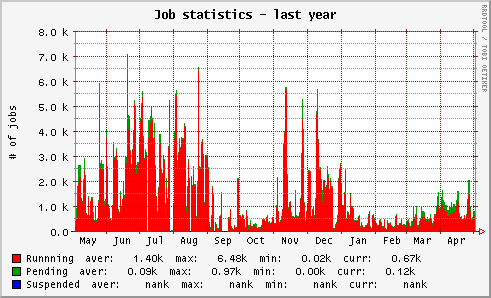
\includegraphics[scale=.44, angle=0]{lsf_c2cms_oneyear.eps}
\caption{CMS number of running and pending transfers during one year}
\label{fig:cmsNbJobs}
\end{figure}

Figure \ref{fig:cmsNbJobs} shows a graph of the number of concurrent I/O
tranfers taking place on the system for a full year for the CMS experiments
production CASTOR setup. When the number of transfers goes higher than the
total number of available slots on the disk servers, exceeding requests were
properly queued in the scheduling system. In this instance and during other
challenges, CASTOR proved able to sustain more than 5000 concurrent transfers and
30 000 pending ones.

%-------------------------------------------------------------------------
\subsection{Internal Data Challenges}

Internal data challenges are performed on a dedicated CASTOR instance
and target specific usage patterns, features, and boundary conditions
of the CASTOR software. They are run under the control of the CASTOR
development team and allow observation of the system under
heavy load so that it can be optimized by tuning its various parameters.
The incoming traffic is generated by scripts, which are able to simulate
the different activities that are foreseen in the Tier 0.
As already introduced in Figure \ref{fig:rates},
four different concurrent activities are taking place:
the raw data transfer from the DAQ (Data acquisition)
buffers, the transfer from the Tier 0 buffer to the reconstruction
farm, the export to the Tier 1 sites through the Grid, and the tape migration.

\begin{figure}[htbp]
\centering
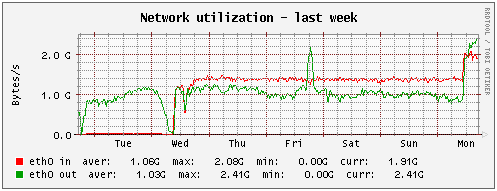
\includegraphics[scale=.6, angle=0]{DAQ_T0_Tape_oneweek.eps}
\caption{Tier 0 data-taking simulation}
\label{fig:itdc1}
\end{figure}

Figure \ref{fig:itdc1} shows the outcome of one week of data acquisition,
including the migration to tape. For this challenge, 100 CPU
nodes have been used as sources, and the CASTOR system has been configured with
48 disk servers with a total of 240~TB and 28 tape drives.
In this configuration the system sustained an average
throughput of 1~GB/s and demonstrated that it could sustain over 2~GB/s for
hours, as shown by the last part of the plot.

Disk servers have been tuned at the kernel and the filesystem level to increase
the throughput of their RAID (Redundant Array of Inexpensive Disks) subsystems.
It has been demonstrated that a standard diskserver, with 24 physical disks
mounted on 3 RAID controllers using the XFS filesystems, can sustain concurrent
inbound and outbound throughput of 70~MB/s using the CASTOR RFIO protocol.

Modern tape drives can deliver between 100 and 120~MB/s of throughput, according to their specifications.
Taking into accounts mount times and tape marks, this results in a 70 to 90~MB/s available data rate,
depending on the average file size.
The CASTOR tape system is able to use all this bandwidth.
However, within a global context, the disk cache scheduling mechanism imposes further constraints on 
the data rates. The typical average data writing rate experienced in a CASTOR production environment
is in the range of 40 to 60~MB/s. This still provides a safe margin to sustain the expected 
data taking requirements of the LHC.

